
%(BEGIN_QUESTION)
% Copyright 2009, Tony R. Kuphaldt, released under the Creative Commons Attribution License (v 1.0)
% This means you may do almost anything with this work of mine, so long as you give me proper credit

Følsomheten og lineariteten i et pneumatisk kraftbalanseinstrument kan forbedres ved å legge til et \textit{pneumatisk forsterkerrelé} som forsterker responsen fra flapper/nozzle-enheten.  Med andre ord: en forsterker i systemet øker systemets \textit{forsterkning}.  Forklar steg for steg hva som skjer i systemet under når kraft påføres armen med tommelen:

$$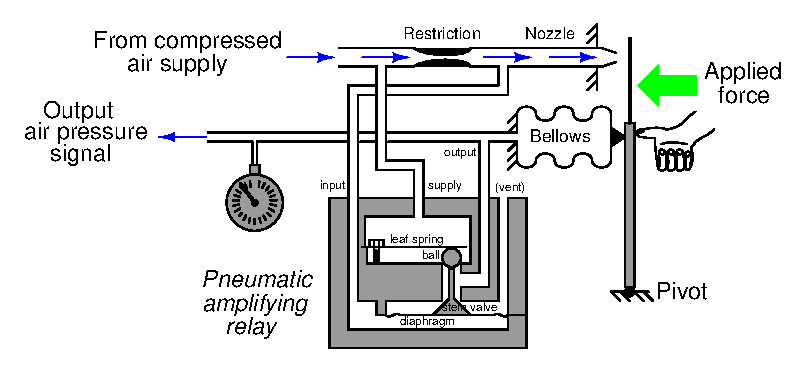
\includegraphics[width=15.5cm]{i00201x01.eps}$$

\vskip 10pt

Avgjør også om mekanismen fortsatt vil gi samme utgangstrykk for en gitt påført kraft uten forsterkerreléet.  Hvis reléet fjernes, blir utgangstrykket høyere enn før, lavere enn før eller likt som før ved samme kraft?

$$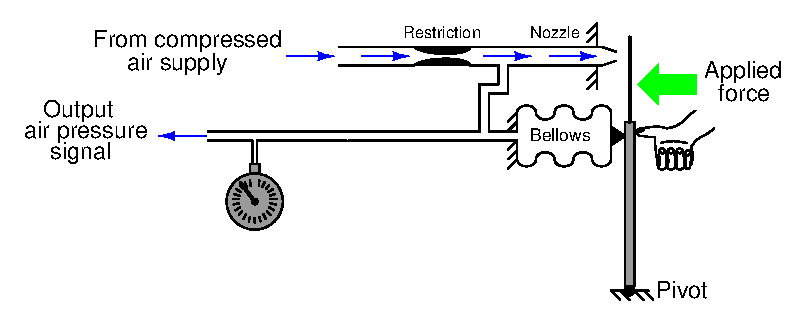
\includegraphics[width=15.5cm]{i00201x05.eps}$$

\vskip 10pt

Utfordringsspørsmål: hvis vi reduserer diameteren i strupingen (orifice) slik at mindre luft strømmer gjennom dysen, blir utgangstrykket høyere, lavere eller likt som før ved samme påførte kraft?

\underbar{file i00201}
%(END_QUESTION)





%(BEGIN_ANSWER)

Det viste pneumatiske forsterkerreléet er typen som ofte brukes i Foxboro-instrumenter.  Det er ikke den eneste relédesignen, men en vanlig variant.

$$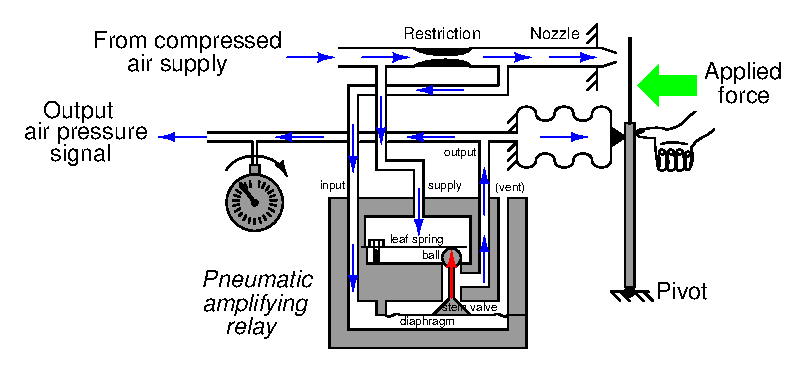
\includegraphics[width=15.5cm]{i00201x02.eps}$$

Hvis armen skyves mot dysen av en ytre kraft, skjer følgende:

\begin{itemize}
\item{} Trykket oppstrøms dysen øker når bafflen gjør dysen mer strupende.
\item{} Dette trykket går inn i reléets ``input'' og presser relémembranen \textit{opp}.
\item{} Membranen løftes, stammeventilen går nærmere setet, og kuleventilen løftes av setet.
\item{} Når kula løftes, slipper mer forsyningsluft inn i området mellom kule og stamme.
\item{} Når stammeventilen lukker mot setet, blir passasjen fra mellomområdet til vent port mer strupet.
\item{} Som resultat av de to foregående punktene øker utgangstrykket til belgen kraftig.
\item{} Belgen utvider seg og skyver armen mot høyre.
\item{} Bafflen flyttes mot høyre til systemet når likevekt med tommelkraften.
\end{itemize}

Reléets virkemåte kan kreve mer forklaring: ``input''-trykket fra dyserøret virker på hele membranarealet og skaper en oppadgående kraft.  Siden kammeret over membranen er ventilert (atmosfærisk trykk), bygges det ikke opp tilsvarende motkraft ovenfra:

$$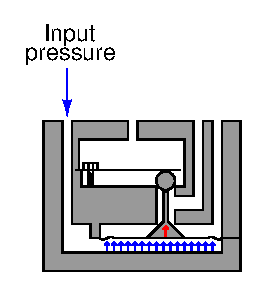
\includegraphics[width=15.5cm]{i00201x03.eps}$$

Kraften løfter kuleventilen og lukker den koniske stammeventilen, altså åpner for mer forsyningsluft inn og struper utlufting ut:

$$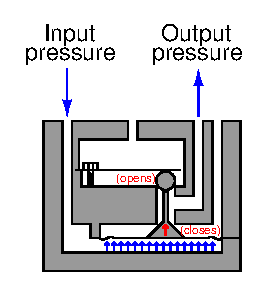
\includegraphics[width=15.5cm]{i00201x04.eps}$$

Den eneste vesentlige motkraften mot membranens bevegelse er en liten bladfjær mot kula.  Fjæren er svak, så små endringer i inngangstrykk gir store endringer i utgangstrykk.  Reléet har altså høy \textit{forsterkning}.

Pneumatiske reléer som dette har samme rolle som operasjonsforsterkere i elektronikk: forsterkere med høy intern forsterkning brukt i negative tilbakekoblingsløkker for å få en lavere og nesten lineær totalforsterkning.  I dette eksemplet blir resultatet (baffle, dyse, arm, relé og belg) et kraftbalansesystem som reagerer aggressivt på ytre kraft på armen.

\vskip 10pt

Tilstedeværelse eller fravær av reléet endrer \textit{ikke} trykk/kraft-forholdet i mekanismen.  Reléet øker bare følsomheten for små kraftendringer og øker responshastigheten.

\vskip 10pt

Svar på utfordringen: å gjøre orifice smalere reduserer luftstrømmen, men endrer ikke trykk/kraft-forholdet.  Dette er fortsatt et kraftbalansesystem der belgkraft må være lik påført kraft ved likevekt, og belgkraften bestemmes av dysetrykket ($F = PA$), ikke av luftstrømmen.

\vskip 10pt

Det bør også nevnes at reléets eksakte forsterkning ($\Delta P_{out} \over \Delta P_{in}$) er lite viktig så lenge den er stor nok.  Dette er analogt med at op-ampens åpen-sløyfe-forsterkning vanligvis er underordnet totalforsterkningen i en negativ tilbakekoblingskrets.

\vskip 10pt

For å endre trykk/kraft-forholdet må man endre tilbakekoblingskomponentene: enten effektivt belgareal eller momentarmen hvor belgen virker.


%(END_ANSWER)





%(BEGIN_NOTES)


%INDEX% Basics, pneumatics: force-balance mechanism

%(END_NOTES)

